\documentclass[compress]{beamer}

\usepackage[utf8]{vntex}
\usepackage{longtable}
\usepackage{amsmath}
\usepackage{amsmath}
\usepackage{amsfonts}
\usepackage{amssymb}
\usepackage[utf8]{inputenc}
\usepackage[absolute,overlay]{textpos}

\usepackage{listings}
\lstset{
	language = Java,
	frame = single,
	tabsize = 3
}

\usetheme{Warsaw}
%\usetheme{Antibes}
%\usecolortheme{spruce}
%\setbeamercolor{structure}{fg=cyan!90!blue}

\expandafter\def\expandafter\insertshorttitle\expandafter{%
    \insertshorttitle\hfill%
    \insertframenumber\,/\,\inserttotalframenumber}
      
\AtBeginSection[] % Do nothing for \section*
{
\begin{frame}
\tableofcontents[currentsection]
\end{frame}
}
\AtBeginSubsection[] % Do nothing for \section*
{
\begin{frame}
\tableofcontents[currentsection, currentsubsection]
\end{frame}
}

\title[Mạng Google Inception]{Mạng Google Inception trong bài toán phân loại} 

\author[Nguyễn Tuấn Đạt, Đặng Quang Trung, Phan Anh Tú]{
Sinh viên thực hiện\\
Nguyễn Tuấn Đạt - 20130856\\
Đặng Quang Trung - 20134145\\
Phan Anh Tú - 20134501 \\[0.4cm]
Giảng viên \\
TS. Đinh Viết Sang 
}

\begin{document} 
\begin{frame}
\titlepage
\end{frame} 
  
\begin{frame}{Nội dung trình bày}
\tableofcontents
\end{frame}
\section{Giới thiệu mạng neuron nhân tạo và học sâu}
\subsection{Mạng neuron nhân tạo}
\begin{frame}{Mạng neuron nhân tạo}
\begin{itemize}
\item Mạng neuron nhân tạo là một mô hình tính toán mô phỏng các hệ thống tương tự mạng neuron sinh học.
\item Mỗi neuron thực hiện một tính toán cục bộ nhận đầu vào và đưa ra đầu ra tương ứng.
\item  Chức năng của một  mạng neuron được xác định bởi :
\begin{itemize}
\item Kiến trúc
\item Đặc tính vào ra
\item Chiến lược học
\item Dữ liệu học 
\end{itemize}
\end{itemize}
\end{frame}
\subsection{Học sâu}
\begin{frame}{Học sâu}
Học sâu là một nhánh của học máy trên cơ sở một tập các thuật toán nhằm cố gắng mô hình hóa trừu tượng mức cao trong dữ liệu bởi việc sử dụng với nhiều tầng xử lý. 
\begin{figure}[H]
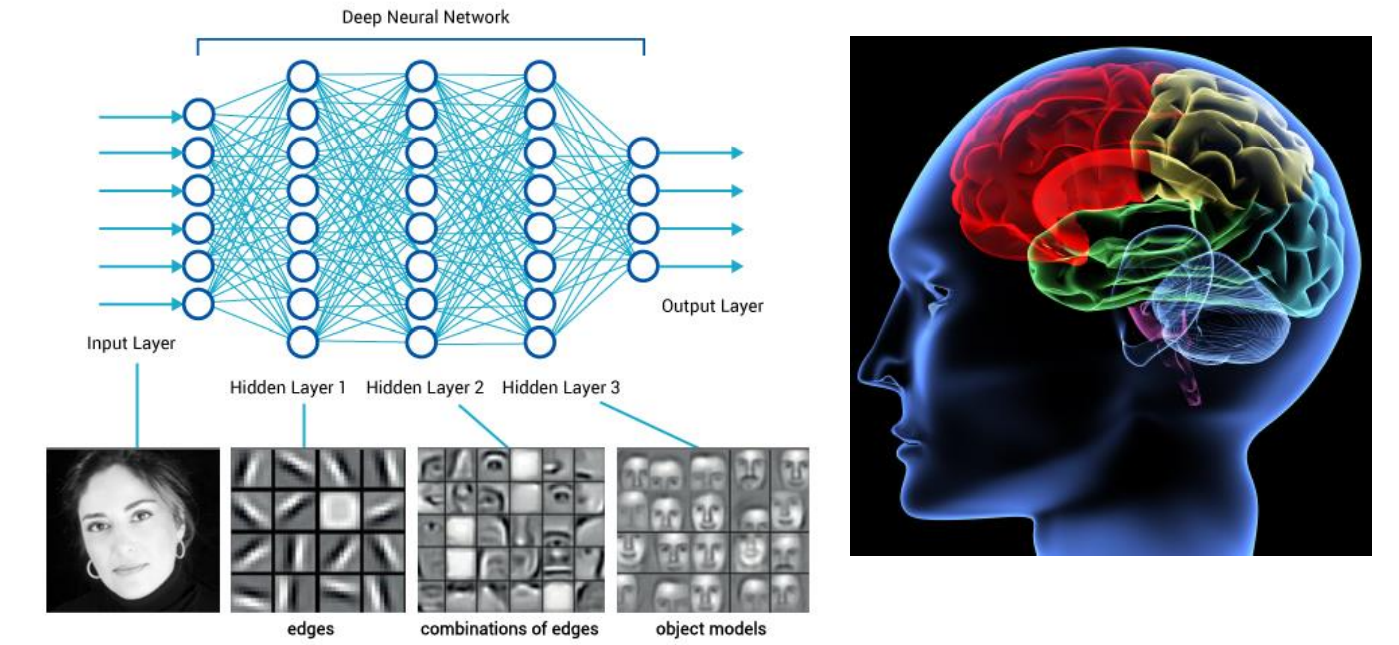
\includegraphics[scale=0.3]{deeplearning.png}
\caption{Mô tả mô hình một mạng neuron học sâu}
\end{figure}
\end{frame}
\begin{frame}{Các thành phần quang trọng trong một mô hình học sâu} 
Các hàm mục tiêu hay được sử dụng: \begin{itemize}
\item sigmoid $\sigma =1/(1+e^-x)$
\item tanh $ tanh(x)$
\item ReLU $ max(0,x)$
\item ELU \abovedisplayskip=0pt\relax
\begin{equation}
\begin{cases}
x \qquad \qquad \qquad  if x>0\\ \alpha (exp(x)-1) \quad if x \leq 0
\end{cases}
\end{equation}
\item Maxout $max(w_1^T x+b_1,w_2^T x+b_2) $

\end{itemize}

\end{frame}
\begin{frame}{Các thành phần quang trọng trong một mô hình học sâu}
\textbf{Kiến trúc mạng}:
\begin{figure}[H]
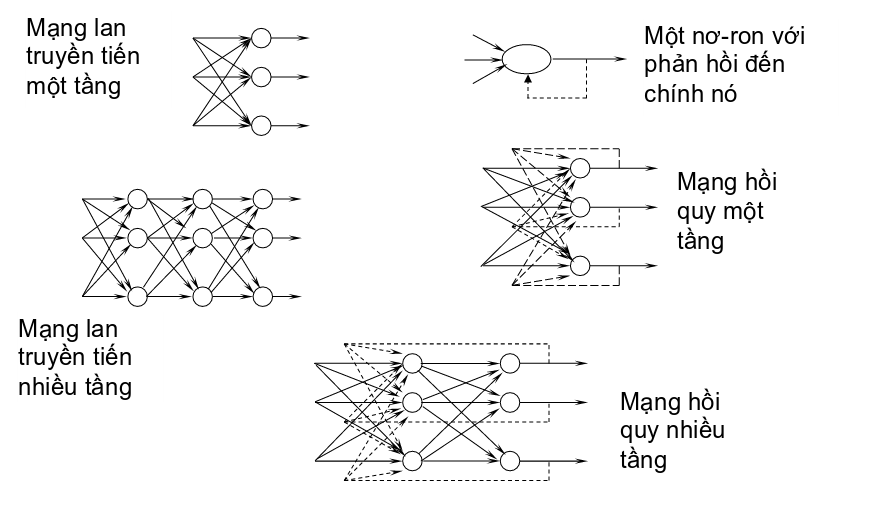
\includegraphics[scale=0.3]{archneuron.png}
\caption{Các kiến trúc mạng neuron điển hình}
\end{figure}
\end{frame}
\begin{frame}{Các thành phần quang trọng trong một mô hình học sâu}
\textbf{Thuật toán học}: Với một mạng neuron lan truyền tiến, hiện tại thuật toán lan truyền ngược vẫn là thuật toán được sử dụng rộng rãi và đem lại hiệu quả cao.\\

\textbf{Chiến lược học}:
\begin{itemize}
\item Stochastic Gradient Descent
\item Mini-batch Gradient Descent
\item Momentum
\item Vanilla
\item Adagrad
\item AdaDelta
\end{itemize}

\end{frame}
\section{Giới thiệu mạng tích chập}
\begin{frame}{Mạng tích chập}
\begin{itemize}
\item Mạng tích chập là một mạng neuron nhân tạo nhiều tầng. Nhưng điều khác biệt chính là ở mỗi neuron trong tầng ẩn của CNN sẽ không kết nối với toàn bộ các neuron thuộc tầng liền trước như mạng thông thường.
\item Trong kiến trúc CNN gồm 3 tầng chính đó là: Convolution Layer, Pooling Layer, Fully-connected Layer.
\end{itemize}

\end{frame}
\subsection{Convolution Layer}
\begin{frame}{Convolution Layer}
Tầng CONV sử dụng một tập các bộ lọc. Mỗi bộ lọc là một không gian nhỏ chiều rộng và chiều cao là các tham số cần chọn, trên toàn bộ chiều sâu của khối đầu vào. Mỗi một bộ lọc sẽ trượt trên toàn kích thước mặt của khối đầu vào và tính toán tại vị trí tương ứng mà bộ lọc trượt qua.
\begin{figure}[H]
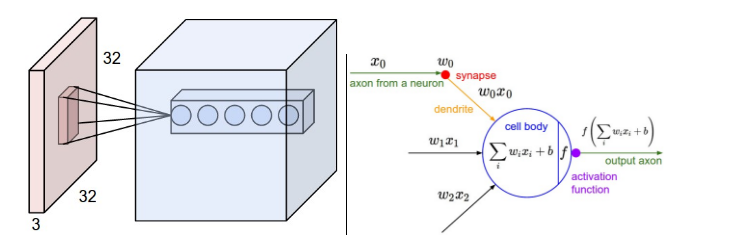
\includegraphics[scale=0.5]{img2.png}
\caption{CONV Layer}
\end{figure}

\end{frame}
\begin{frame}{Convolution Layer}
\begin{itemize}
\item	Không gian số lượng các neurons ở đầu ra được quy định bởi 3 tham số :depth(độ sâu), stride(bước trượt) và mức lề (zero-padding):
\begin{itemize}
\item[1. ] Độ sâu ở đầu ra tương ứng với số lượng bộ lọc được sử dụng.
\item[2. ] Stride là số bước nhảy khi trượt bộ lọc.
\item[3. ] Dữ liệu ở mép các ma trận rất dễ bị mất  dần qua mỗi tầng vì vậy sử dụng một kích thước lề bao quanh đầu vào, giá trị của lề đều bằng 0. 

\end{itemize} 
\item Trong mạng CNN ta luôn chỉ sử dụng một vector trọng số cho các neuron có cùng độ sâu.
\end{itemize}
\end{frame}
\begin{frame}{Ví dụ}
\begin{figure}[H]
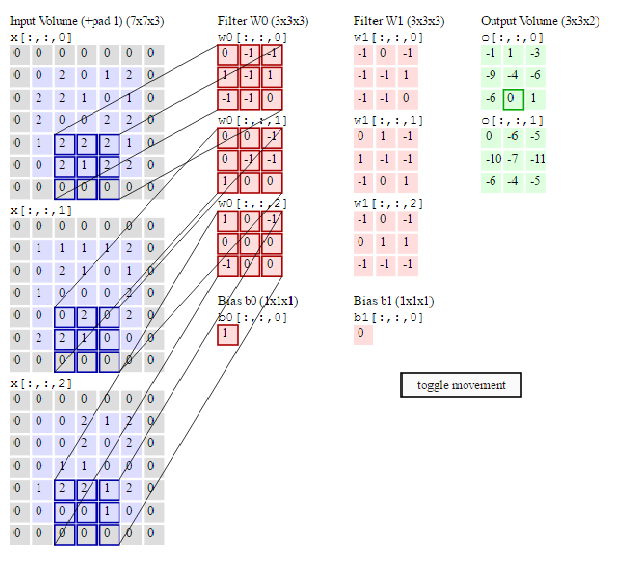
\includegraphics[scale=0.5]{img3.png}
\caption{Ví dụ CONV}
\end{figure}
\end{frame}
\subsection{Pooling Layer}
\begin{frame}{Pooling Layer}
\begin{figure}[H]
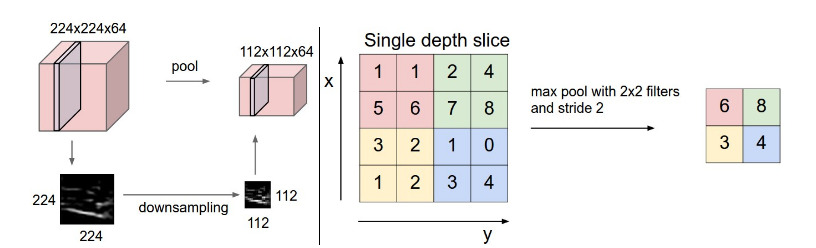
\includegraphics[scale=0.5]{img4.png}
\caption{Ví dụ CONV}
\end{figure}
\end{frame}
\subsection{Kiến trúc tổng quát}
\begin{frame}{Kiến trúc CNN}
\small{
\textbf{INPUT -> [[CONV -> RELU]*N -> POOL?]*M -> [FC -> RELU]*K -> FC}
}

\end{frame}


\section{Google Inception}
\subsection{Inception Module}
\begin{frame}{Inception Module naive version}
\begin{itemize}
\onslide<1->{\item Thay vì nhìn dữ liệu theo 1 cách ở mỗi tầng thì sẽ nhìn dữ liệu theo nhiều cách}
\onslide<2->
\begin{figure}[H]
%\centering
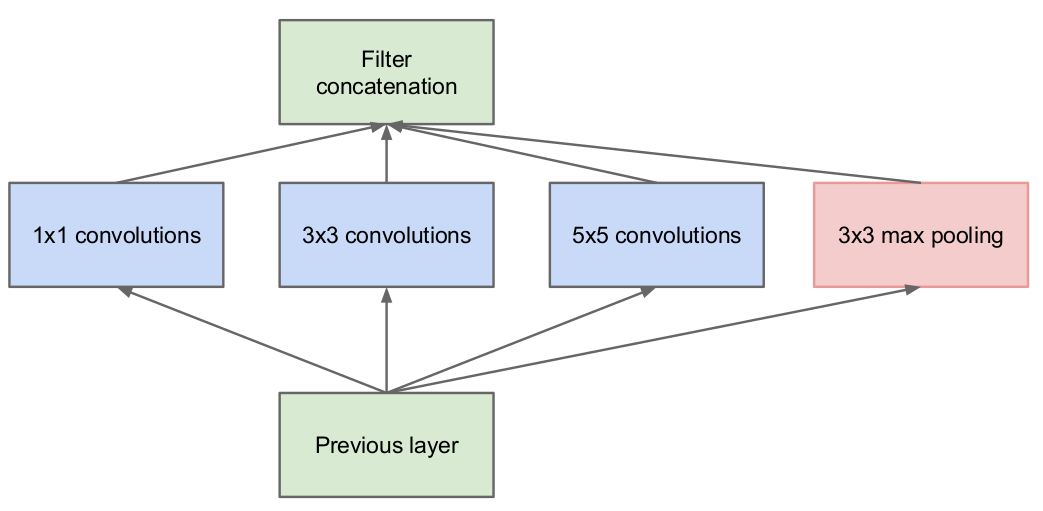
\includegraphics[scale=0.25]{inception_naive.png}
\end{figure}
\item Output của các tầng $1 \times 1$, $3 \times 3$, $5 \times 5$ là $H \times W \times C_1$, $H \times W \times C_3$, $H \times W \times C_5$  \onslide<3-> $\rightarrow$ output $H \times W \times (C_1+C_3+C_5)$

\end{itemize}
\end{frame}


\begin{frame}{Inception module với kỹ thuật giảm chiều}
\begin{itemize}
\onslide<1->{\item Để giảm chi phí tính toán, trước khi tính toán với các filter lớn ($3\times 3$ và $5 \times 5$) sử dụng các filter kích thước $1 \times 1$ để giảm chiều dữ liệu sẽ giúp cho giảm chi phí tính toán}
\onslide<2->{
\begin{figure}[H]
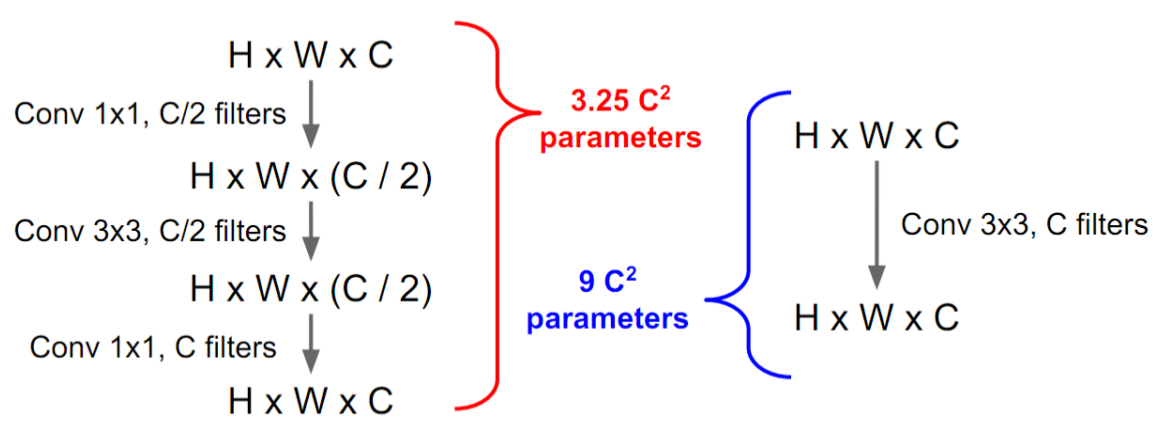
\includegraphics[scale=0.3]{reduce_1x1.png}
\end{figure}}
\end{itemize}
\end{frame}

\begin{frame}{Inception module với kỹ thuật giảm chiều}
\begin{figure}[H]
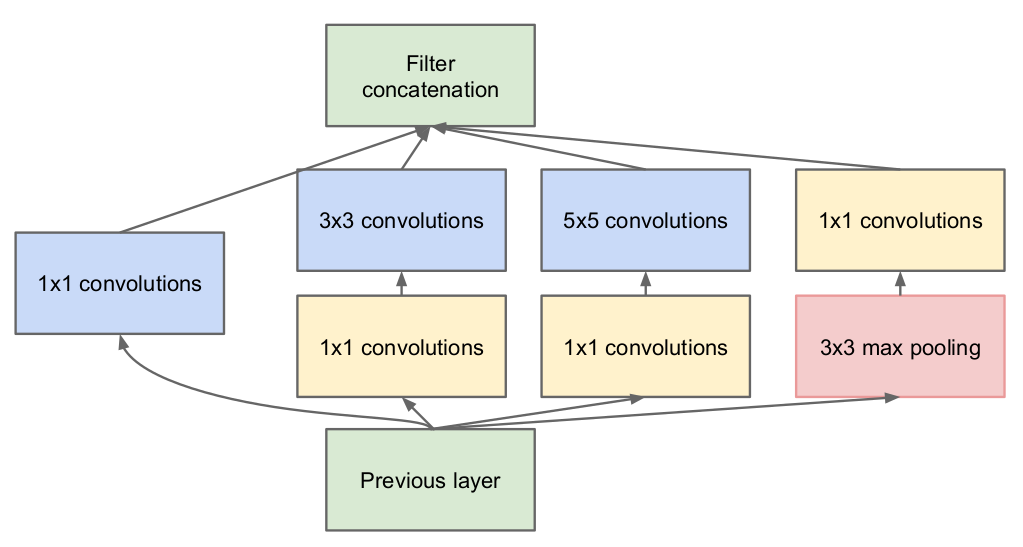
\includegraphics[scale=0.33]{inception_reduce.png}
\end{figure}
\end{frame}

\subsection{Cải tiến Inception Module}
\begin{frame}{Phân rã tầng convolution}
\begin{itemize}
\onslide<1->{\item Đặt 2 tầng Convolution (với kích thước filter mỗi tầng là $3 \times 3$ và stride là 1) cạnh nhau} 
\onslide<2->{\item Mỗi neuron thuộc tầng convolution thứ 2 sẽ nhìn vào một vùng kích thước $5 \times 5$ trong khối đầu vào của tầng thứ convolution thứ nhất} 
\onslide<3->{\begin{figure}[H]
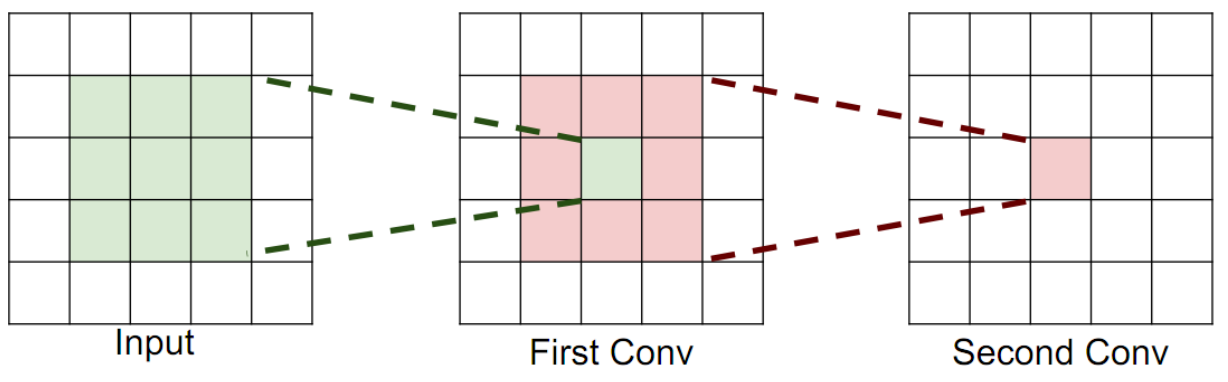
\includegraphics[scale=0.33]{2conv3x3.png}
\end{figure}}
\end{itemize}
\end{frame}

\begin{frame}{Hiệu quả của việc phân rã}
\begin{itemize}
\onslide<1->\item Một khối đầu vào có kích thước $H \times W \times C$ 
\begin{itemize}
\onslide<2->\item Một tầng convolution có $C$ filter kích thước $5 \times 5$ (với stride = 1 và padding để bảo toàn kích thước đầu vào) 
\begin{itemize}
\onslide<3->\item Số lượng tham số sẽ là: $C \times (5 \times 5 \times C) = 25C^2$ 
\onslide<4->\item Khối lượng tính toán là: $(H \times W \times C) \times (7 \times 7 \times C) = 25HWC^2$ 
\end{itemize}
\onslide<2->\item 2 tầng convolution có $C$ filter kích thước $3 \times 3$ ở mỗi tầng (với stride = 1 và padding để bảo toàn kích thước đầu vào) 
\begin{itemize}
\onslide<3->\item số lượng tham số sẽ là : $2 \times C \times (3 \times 3 \times C) = 18C^2$
\onslide<4->\item khối lượng tính toán là: $2 \times (H \times W \times C) \times (3 \times 3 \times C) = 18HWC^2$
\end{itemize}
\end{itemize}
\onslide<5-> \textbf{Phân rã 1 tầng $3\times 3$ thành 2 tầng $2 \times 2$ ???}
\end{itemize}
\end{frame}

\begin{frame}{Phân rã $2\times 2$ ??} 
\begin{itemize}
\onslide<1->\item Khối đầu vào có kích thước $H \times W \times C$ 
\begin{itemize}
\onslide<2->\item 2 tầng convolution có $C$ filter kích thước $2 \times 2$ (với stride = 1 và padding để bảo toàn kích thước đầu vào) 
\begin{itemize}
\onslide<3->\item Số lượng tham số sẽ là: $2 \times C \times (2 \times 2 \times C) = 8C^2$ 
\onslide<4->\item Khối lượng tính toán (số lượng phép toán) là: $2 \times (H \times W \times C) \times (2 \times 2 \times C) = 8HWC^2$
\end{itemize}
\onslide<2->\item 1 tầng convolution có $C$ filter kích thước $1 \times 3 $ + 1 tầng convolution có $C$ filter kích thước $3 \times 1$ (cả 2 tầng đều có tham số stride = 1 và padding để bảo toàn kích thước đầu vào)
\begin{itemize}
\onslide<3->\item Số lượng tham số là: $C \times 1 \times 3 \times C+ C \times 3 \times 1 \times C = 6C^2$ 
\onslide<4->\item khối lượng tính toán là: $(H \times W \times C) \times (1 \times 3 \times C) + (H \times W \times C) \times (3 \times 1 \times C) = 6HWC^2$
\end{itemize}
\end{itemize}
\end{itemize}
\end{frame}

\subsection{Inception v4}
\begin{frame}{Kiến trúc Inception v4}
\begin{figure}[H]
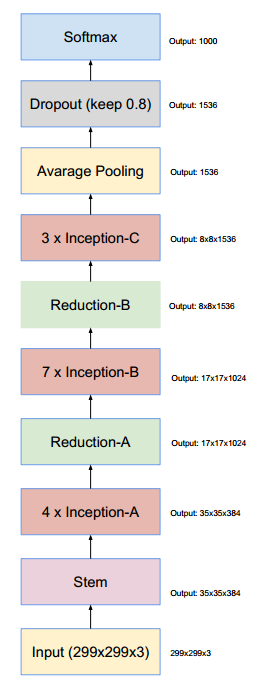
\includegraphics[scale=0.3]{inceptionv4.png}
\end{figure}
\end{frame}

\begin{frame}{Inception-A}
\begin{figure}[H]
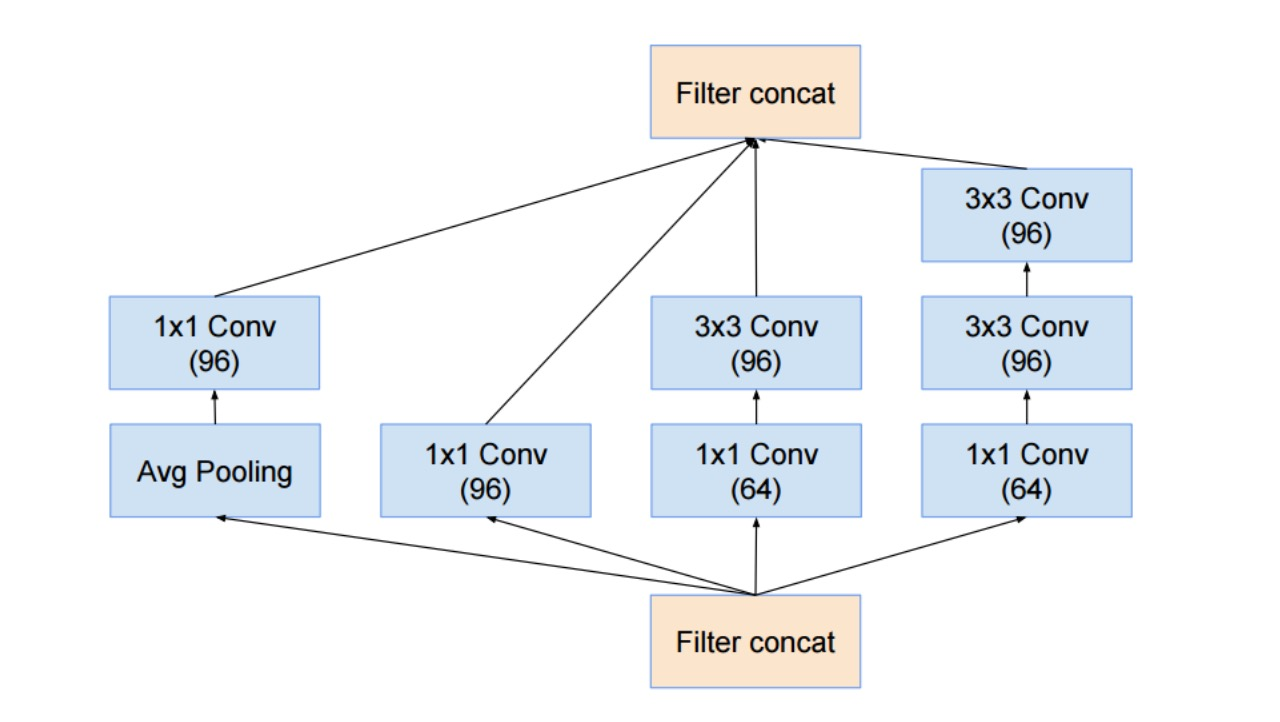
\includegraphics[scale=0.29]{inceptionA.jpg}
\end{figure}
\end{frame}

\begin{frame}{Inception-B}
\begin{figure}[H]
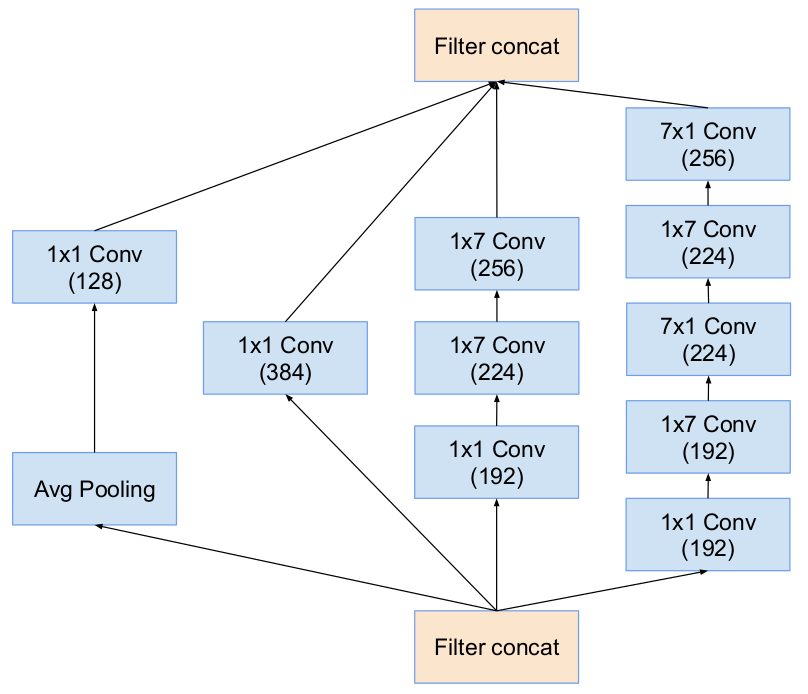
\includegraphics[scale=0.3]{inceptionB.png}
\end{figure}
\end{frame}

\begin{frame}{Inception-C}
\begin{figure}[H]
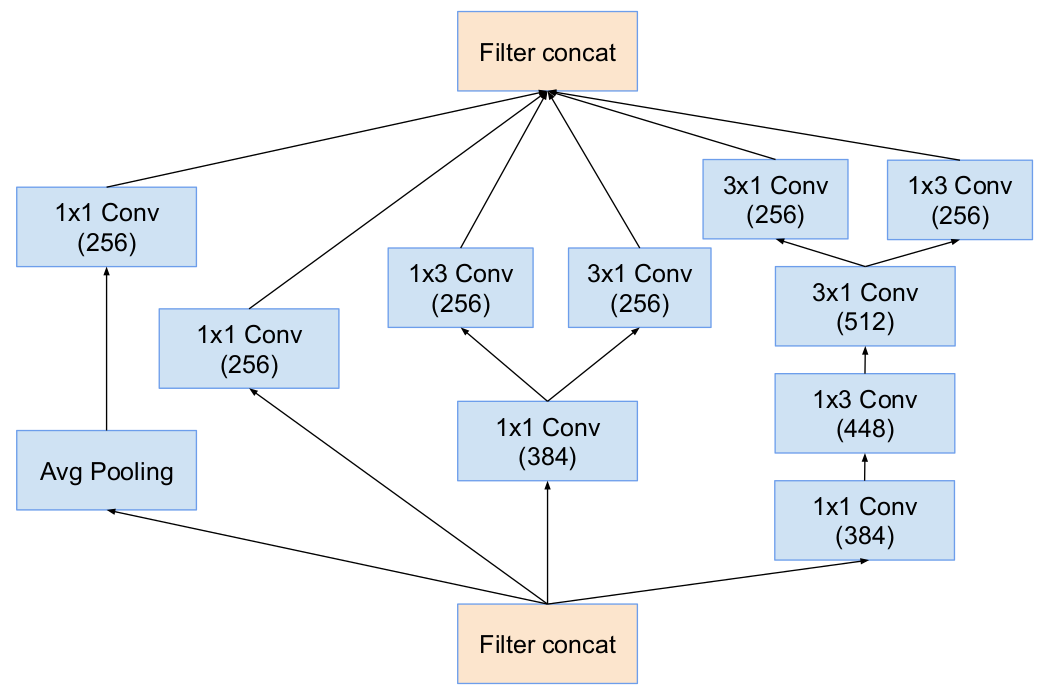
\includegraphics[scale=0.29]{inceptionC.png}
\end{figure}
\end{frame}

\begin{frame}{Reduce-B}
\begin{figure}[H]
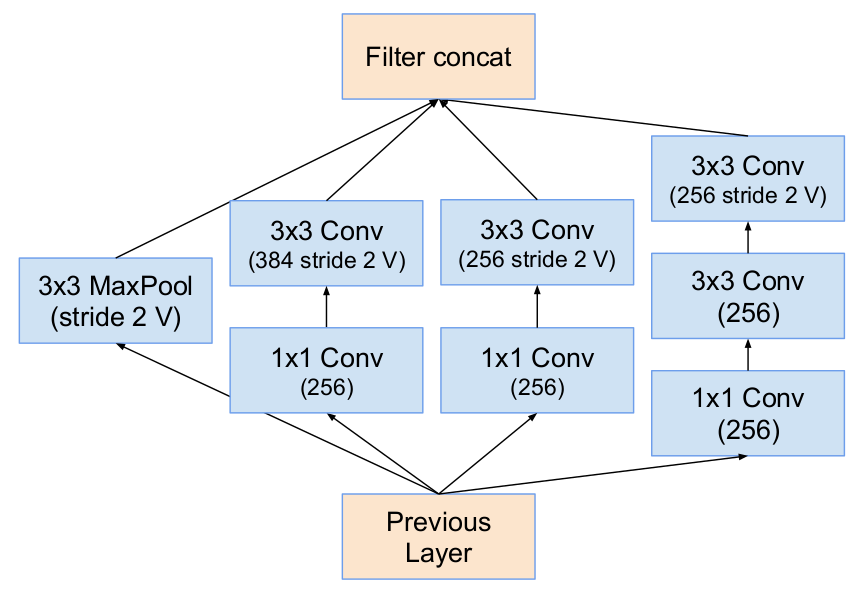
\includegraphics[scale=0.3]{reduceB.png}
\end{figure}
\end{frame}
\begin{frame}{Cảm ơn thầy và các bạn đã lắng nghe}

\includegraphics[scale=0.6]{thanks.jpg}
\end{frame}
\begin{frame}{Tài liệu tham khảo}
\begin{thebibliography}{9}
\bibitem{googlenet} C. Szegedy, W. Liu, Y. Jia, P. Sermanet, S. Reed, D. Anguelov, D. Erhan, V. Vanhoucke, and A. Rabinovich. \textit{Going deeper with convolutions}

\bibitem{rethinking} C. Szegedy, V. Vanhoucke, S. Ioffe, J. Shlens, and Z. Wojna. \textit{Rethinking the inception architecture for computer vision}

\bibitem{inceptionv4} C. Szegedy, S. Ioffe, and V. Vanhoucke. \textit{Inception-v4, Inception-ResNet and the Impact of Residual Connections on Learning}

\bibitem{slidesangdv} Slide DeepLearning, Thầy Đinh Viết Sang 

\bibitem{slidekhoattq} Slide mạng neuron, Thầy Thân Quang Khoát

\bibitem{deeplearningbook}  http://www.deeplearningbook.org/
\bibitem{CNN} Mạng CNN ,http://cs231n.github.io/convolutional-networks/
\bibitem{inceptionsource} Inception v4 in keras 
\end{thebibliography}

\end{frame}
\end{document}
